\documentclass[12pt,a4paper]{article} 

\usepackage[spanish]{babel} 
\usepackage[utf8]{inputenc}
\usepackage[numbers,sort&compress]{natbib}
\usepackage{graphicx} 
\usepackage{graphics} 
\usepackage{amsfonts}
\usepackage[left=2cm,right=2cm,top=2cm,bottom=2cm]{geometry}
\usepackage{listings}
\usepackage[usenames,dvipsnames]{color}
\usepackage{subfig}
\usepackage{natbib}
\author{Paola Lizbeth Vázquez}

\title{Matemáticas Computacionales \\ Práctica 3: Método de Bisección } 
\author{Profesor: Ángel Isabel Moreno Saucedo \\ Alumno: Paola Lizbeth Vázquez Leal \\ Semestre Febrero - Junio 2021}
\date{}

\begin{document}
\maketitle
Práctica 3
\section{Introducción}

En esta actividad se busca encontrar la cantidad de iteraciones que realiza el programa para encontrar los ceros de las funciones en base al método de bisección.

\section{Método de bisección.}

Se considera uno de los métodos más sencillos al momento de resolver ecuaciones de una variable. Este metdo trata de los valores intermedios, donde establece que toda función confinua en $f$ dentro de un intervalo cerrado $[a,b]$  toma todos los valores que se encuentran en $f(a)$ y $f(b)$. 

Si $f(a)$ y $f(b)$ son opuestos (por los signos) el valor cero se convierte en un valor intermedio entre estos dos, por lo que se puede decir que existe un x estrella ($\mathbf{x^*}$) en ese intervalo que cumple lo siguiente: $\mathbf{f(x^*)=0}$.
Con ello se puede asegurar la existencia de al menos una solución a la función dada.


El metodo se aplica de la siguiente manera: 
suponer que dentro del intervalo $[a,b]$ hay un cero (raíz) de $f$. se calcula el punto medio con la siguiente formula:
\begin{equation}
 m= \frac{(a+b)}{2}
\end{equation}

Seguido de obtener nuestro punto medio podemos calcular $f(m)$, si esta funcion es igual a 0 ($f(m)=0$) se puede decir que se ha encontrado la solucion, en caso de no ser así se corrobora que $f(m)$ tenga signo opuesto a $f(a)$. Asi se puede redefinir el intervalo como $[a,m]$ o $[m,b]$ según sea el caso. Seguido se vuelve a emplear el mismo meétodo, encerrando la solucion en un intervalo más pequeño hasta obtener el esperado. \citep{Metnum}

\citep{repositorio} A continuación se puede apreciar el método explicado. 

\begin{figure}
\centering
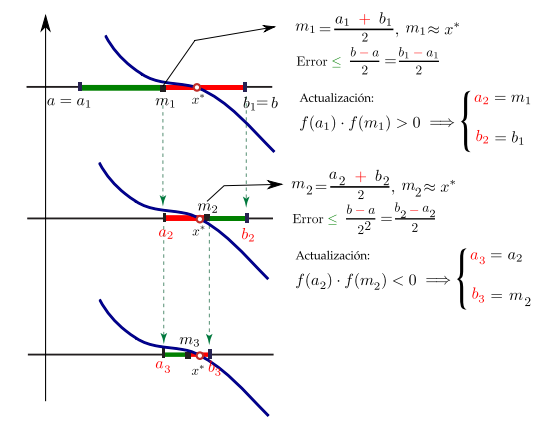
\includegraphics[scale=0.8]{Método_bisección}
\caption{Método de solución para la bisección.}
\end{figure}

\textbf{El error de estimación:}
El error exacto en el k-ésimo
paso es $\mathbf{|m_k -x^*|}$.
 Geométricamente se puede ver que
esto es menos que la mitad del intervalo $[a_k ,b_k ]$, es decir

\begin{equation}
\mathbf{|m_k -x^*|} \leq \frac{b_k - a_k}{2} = \frac{b-a}{2^k}
\end{equation}

\begin{figure}
\centering
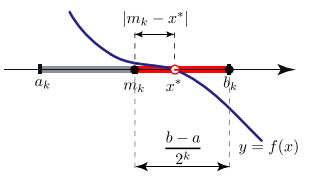
\includegraphics[scale=0.8]{error de est}
\caption{Estimación de error.}
\end{figure}

\newpage
\section{Funciones}
\subsection{Función 1}
$\mathbf{ x^3 = 0}$ Usando bisección con el intervalo $[-0.2, 0.1]$.
La tolerancia dada para esta funcion fue de $0.000001$ por lo que la función necesito de 18 iteraciones para encontrar los ceros dentro de el intervalo dado. [\ref{funcion1}] \\
 

\begin{tabular}{| c | c | c | c |}
\hline
 & Función 1 & &  \\
\hline
 a          &     b           &    m            &   Error est.  \\ \hline
-0.0500000   &    0.1000000   &   -0.0500000    &   0.0750000   \\   
-0.0500000   &   0.0250000    &   0.0250000     &  0.0375000   \\   
-0.0125000   &    0.0250000   &   -0.0125000    &   0.0187500   \\   
-0.0125000   &    0.0062500   &    0.0062500    &   0.0093750   \\   
-0.0031250   &    0.0062500   &   -0.0031250    &   0.0046875   \\   
-0.0031250   &    0.0015625   &    0.0015625    &   0.0023437   \\   
-0.0007812   &    0.0015625   &   -0.0007812    &   0.0011719   \\   
-0.0007812   &    0.0003906   &    0.0003906    &   0.0005859   \\   
-0.0001953   &    0.0003906   &   -0.0001953    &   0.0002930   \\   
-0.0001953   &    0.0000977   &    0.0000977    &   0.0001465   \\   
-0.0000488   &    0.0000977   &   -0.0000488    &   0.0000732   \\   
-0.0000488   &    0.0000244   &    0.0000244    &   0.0000366   \\   
-0.0000122   &    0.0000244   &   -0.0000122    &   0.0000183   \\   
-0.0000122   &    0.0000061   &    0.0000061    &   0.0000092   \\   
-0.0000031   &    0.0000061   &   -0.0000031    &   0.0000046   \\   
-0.0000031   &    0.0000015   &    0.0000015    &   0.0000023   \\   
-0.0000008   &    0.0000015   &   -0.0000008    &   0.0000011   \\   
-0.0000008   &    0.0000004   &    0.0000004    &   0.0000006   \\ \hline
                          
 \end{tabular}
 
 
\begin{figure}
\centering
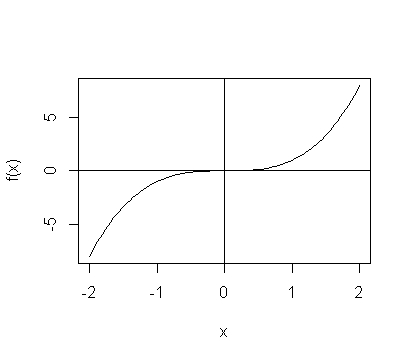
\includegraphics[scale=0.9]{funcion1}
\caption{Su cero se encuentra en [ -0.2 , 0.1 ] es approx:  3.814697e-07 con error <= 5.722046e-07}
\label{funcion1}
\end{figure} 
 
\subsection{Función 2}
$\mathbf{f(x)= x^5 - 100*x^4 + 3995*x^3 - 79700*x^2 + 794004*x - 3160075 }$ usando bisección con [17, 22.2]. La tolerancia dada para esta funcion fue de $0.000001$ por lo que la función necesito de 22 iteraciones para encontrar los ceros dentro de el intervalo dado. [\ref{funcion2}] \\


\begin{figure}
\centering
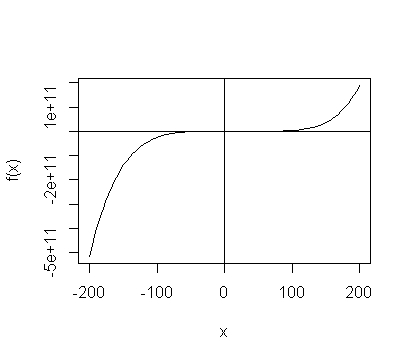
\includegraphics[scale=0.9]{funcion2}
\caption{Su cero se encuentra en en [ 17 , 22.2 ] es approx:  17.84636 con error <= 6.198883e-07}
\label{funcion2}
\end{figure}
 

\begin{tabular}{| c | c | c | c |}
\hline
 & Función 2 & &  \\
\hline
a       &             b        &       m        &   Error est.  \\ \hline
 17.0000000  &    19.6000000   &   19.6000000   &   1.3000000 \\     
 17.0000000  &    18.3000000   &   18.3000000   &   0.6500000 \\     
 17.6500000  &    18.3000000   &   17.6500000   &   0.3250000 \\     
 17.6500000  &    17.9750000   &   17.9750000   &   0.1625000 \\     
 17.8125000  &    17.9750000   &   17.8125000   &   0.0812500 \\     
 17.8125000  &    17.8937500   &   17.8937500   &   0.0406250 \\     
 17.8125000  &    17.8531250   &   17.8531250   &   0.0203125 \\     
 17.8328125  &    17.8531250   &   17.8328125   &   0.0101562 \\     
 17.8429687  &    17.8531250   &   17.8429687   &   0.0050781 \\     
 17.8429687  &    17.8480469   &   17.8480469   &   0.0025391 \\     
 17.8455078  &    17.8480469   &   17.8455078   &   0.0012695 \\     
 17.8455078  &    17.8467773   &   17.8467773   &   0.0006348 \\     
 17.8461426  &    17.8467773   &   17.8461426   &   0.0003174 \\     
 17.8461426  &    17.8464600   &   17.8464600   &   0.0001587 \\     
 17.8463013  &    17.8464600   &   17.8463013   &   0.0000793 \\     
 17.8463013  &    17.8463806   &   17.8463806   &   0.0000397 \\     
 17.8463409  &    17.8463806   &   17.8463409   &   0.0000198 \\     
 17.8463608  &    17.8463806   &   17.8463608   &   0.0000099 \\     
 17.8463608  &    17.8463707   &   17.8463707   &   0.0000050 \\     
 17.8463608  &    17.8463657   &   17.8463657   &   0.0000025 \\     
 17.8463633  &    17.8463657   &   17.8463633   &   0.0000012 \\     
 17.8463645  &    17.8463657   &   17.8463645   &   0.0000006 \\ \hline
\end{tabular}


\newpage
\subsection{Función 3}
$\mathbf{x^3-2*x-5=0}$ Esta función solo tiene una raíz en el punto $[2.094564, 0]$
Dependiendo el intervalo que se elija para encontrar las raices es la cantidad de iteraciones. [\ref{funcion3}]

\begin{figure}
\centering
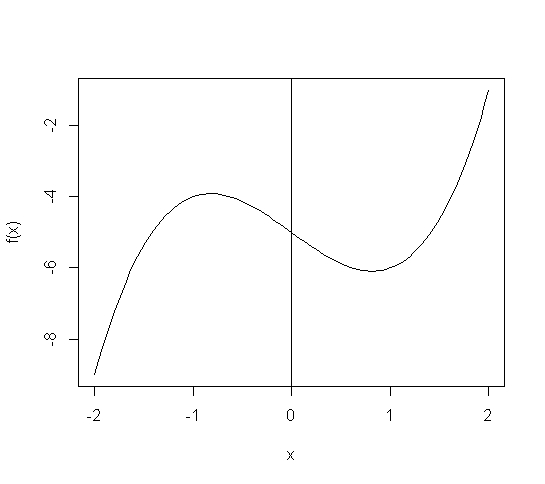
\includegraphics[scale=0.8]{funcion3}
\caption{La raíz de la función $\mathbf{x^3-2x-5}$ es 2.094564}
\label{funcion3}
\end{figure}

\bibliography{bibliografia}
\bibliographystyle{plainnat}

\end{document}